\section{Umsetzung}
\label{sec-5}
\fbox{
\parbox{\linewidth}{
	\textit{Ziel des Kapitels:}\\
	Umsetzung erläutern: Wie wurde die Lösungsidee umgesetzt?
}}\\

Im folgenden soll erläutert werden, wie der zuvor erarbeitete Lösungsansatz umgesetzt wurde. Dazu gibt das Kapitel zunächst einen Überblick über das System und die Architektur der Anwendung. Nach einer kurzen Erläuterung zu ''Screen-Captures'' von der HoloLens folgt eine nähere Betrachtung dessen, wie die Hologramme umgesetzt wurden. Schließlich werden Details zur Interaktion und Performance genannt.

\subsection{Aufbau des Systems}
Das System ist als Client-Server-Architektur realisiert, einen Überblick gibt das Schema in Abb. \ref{img:communication-schema}. Ein Server erfasst und verarbeitet die in der Schaltung gemessenen Werte für die Stromstärke. Diese stammen von einem Arduino, der in den Stromkreislauf eingekoppelt ist. Die Applikation auf der HoloLens tritt als Client auf und erfragt die aktuellen Werte vom Server. 
\begin{figure}[H]
	\centering
	\includegraphics[width=1\textwidth]{images/todo.jpg}
	\caption{Schema Kommunikation Schaltung Arduino Server HoloLens}
	\label{img:communication-schema}
\end{figure}

\subsubsection{Client-Server Datenübertragung}
Die Übertragung der Messwerte vom Arduino zur Anwendung ist so konzipiert, dass Änderungen in Echtzeit übermittelt werden, ohne das unnötiger Netzwerktraffic entsteht. Der Client betreibt ein Polling gegen den Server, der jedoch Antworten solange zurückhält, bis ein neuer, vom vorigen abweichender Wert gemessen wurde. Dieses Verhalten veranschaulicht das Sequenzdiagramm in Abbildung \ref{img:Sequenzdiagramm}. Das Vorgehen führt dazu, dass Änderungen durch den Nutzer am Regler der Spannungsquelle ohne wahrnehmbare Verzögerung auf der HoloLens ankommen.

\vspace{8px}
\begin{center}
	\fbox{
		\parbox{0.9\linewidth}{
			\vspace{4px}
			\textbf{Überblick}
			\begin{itemize}[rightmargin=12px, topsep=-12px]
				\setlength{\itemsep}{-1pt}
				\singlespacing
				\item HoloLens erfragt Daten vom Server über HTTP GET-Requests
				\item Anfragen erfolgen asynchron
				\item Server nimmt den Request entgegen und hält eine Antwort solange zurück, bis ein neuer Wert vom Arduino vorliegt
				\item Dadurch kommen neue Daten sehr schnell bei der HoloLens an, der Nutzer sieht die Änderungen auf der Brille sofort, wenn er Änderungen an der Spannungsquelle vornimmt
				\item Dadurch wird zeitliche Einbettung und Kontinuität erreicht
				\item Dabei wird jedoch kein unnötiger Traffic erzeugt, wenn es keine Änderungen gibt
			\end{itemize}
			\vspace{18px}
	}}\\
\end{center}
%\vspace{6px}

\begin{figure}[H]
	\centering
	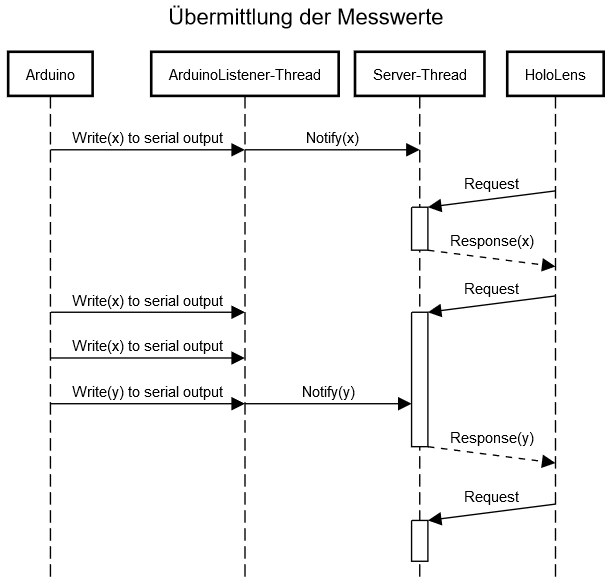
\includegraphics[width=1\textwidth]{images/Sequenzdiagramm.png}
	\caption{Sequenzdiagramm Kommunikation}
	\label{img:Sequenzdiagramm}
\end{figure}

\textit{Server}\\
Der Server besteht aus zwei miteinander kommunizierenden Threads. Ein Thread übernimmt das Lesen und Verarbeiten der Rohdaten, die über die serielle Schnittstelle eintreffen. Bei signifikanten Änderungen wird der zweite Thread mittels einer gemeinsamen, synchronisierten Variablen über die neuen Werte informiert. Dieser beantwortet daraufhin einen ggf. ausstehenden Request vom Client. Ab wann eine Änderung als signifikant gewertet wird, lässt sich über einen Threshold einstellen. Der Server wurde mit Python und der Bibliothek pyserial umgesetzt.\\

\textit{Client}\\
Der Client stellt durch die Nutzung von asynchronen Anfragen sicher, dass die Anfragen nicht blockieren. Unity bietet nur einen Thread, synchrone Anfragen würden daher zu einer Blockierung des Renderprozesses führen und so die Framerate beeinträchtigen. Da die Framerate bei 60 Hz gedeckelt ist und eine Antwort frühestens im nächsten Frame bearbeitet werden kann, beträgt die minimale Antwortzeit ca. 17 ms. Das ist ausreichend, um keine wahrnehmbare Verzögerung aufkommen zu lassen, da die Paketlaufzeit in einem lokalen Netzwerk typischerweise im einstelligen Millisekundenbereich liegt. Eine zusätzliche Wartezeit zwischen Requests kann außerdem eingestellt werden.\\

\subsubsection{Architektur der HoloLens-Anwendung}
Der Hauptteil des Systems besteht in der auf der HoloLens laufenden Applikation. Die Anwendung basiert auf der Unity Engine und wird als UWP App bereitgestellt. Das Schema in Abb. \ref{img:components-schema} gibt einen Überblick über die verschiedenen Komponenten der Anwendung. Deren Aufgaben sind in der darunter zu findenden Tabelle kurz zusammengefasst.

\begin{figure}[H]
	\centering
	\includegraphics[width=1\textwidth]{images/todo.jpg}
	\caption{Schema Komponenten}
	\label{img:components-schema}
\end{figure}


\vspace{8px}
\begin{center}
	\fbox{
		\parbox{0.9\linewidth}{
			\vspace{4px}
			\textbf{Überblick}	
\bgroup
\setlength\extrarowheight{-2pt}
\def\arraystretch{2}
\begin{table}[H]
	\centering
	\begin{tabular}{m{2.5cm}|m{8cm}}
		Komponente & Funktion\\
		\hline
		\hline
		Menu & Hauptmenü, steuert den Ablauf der Anwendung\\
		\hline
		Settings & Lädt und Speichert Einstellungen, bietet Zugang zu den Werten für andere Komponenten und steuert die Einstellungs-Oberfläche\\
		\hline
		Physics & Übernimmt alle physikalischen Berechnungen. Alle relevanten physikalischen Parameter lassen sich konfigurieren.\\
		\hline
		Tracking & Führt durch den Prozess der Positionsbestimmung und setzt den World Anchor\\
		\hline
		Model Anchor & Dient als Anker- und Container-Objekt für die einzelnen Darstellungskomponenten. Dazu gehören: Verdeckungsmodell, Kompass, die Magnetfeldmodelle, die Stromrichtungsindikatoren und das Datenpanel.\\
		\hline
		Webservice & Übernimmt die Kommunikation mit dem Server und gibt erhaltene Daten weiter\\
		\hline
		Interaction & Verarbeitet Input und Ablaufsteuerung, soweit dies nicht an einem konkreten Objekt abgewickelt wird wie z.B. Spracheingabe.\\
	\end{tabular}\caption{\label{tab:components-details} Aufgaben der einzelnen Komponenten}
\end{table}
\egroup
%\vspace{18px}
}}\\
\end{center}
\vspace{6px}

Eine Komponente besteht aus einer Hierarchie von Unity's GameObjects, die mit entsprechenden Skripten versehen sind. Die Komponenten kommunizieren auf unterschiedliche Weise miteinander. Die Behandlung von Events z.B. aufgrund von Nutzereingaben oder neuen Messwerten erfolgt über Callbacks. Manche Komponenten sind auch Singletons, auf die direkt zugegriffen werden kann wie z.B. die Einstellungen. 

\subsection{Darstellungen}
Nachdem die grundlegende Architektur der vorgestellt wurde folgt nun eine genauere Betrachtung der Umsetzung der Darstellungen. Die Ausführungen werden dabei durch Abbildungen in Form von Screenshots unterstützt. Einen ersten Eindruck vermitteln die Fotos in Abb. \ref{img:HL_SS_Intro}. Damit die von der HoloLens stammenden Bilder richtig interpretiert werden können, sind jedoch einige Vorbemerkungen nötig.

\begin{figure}[h!]
	\centering
	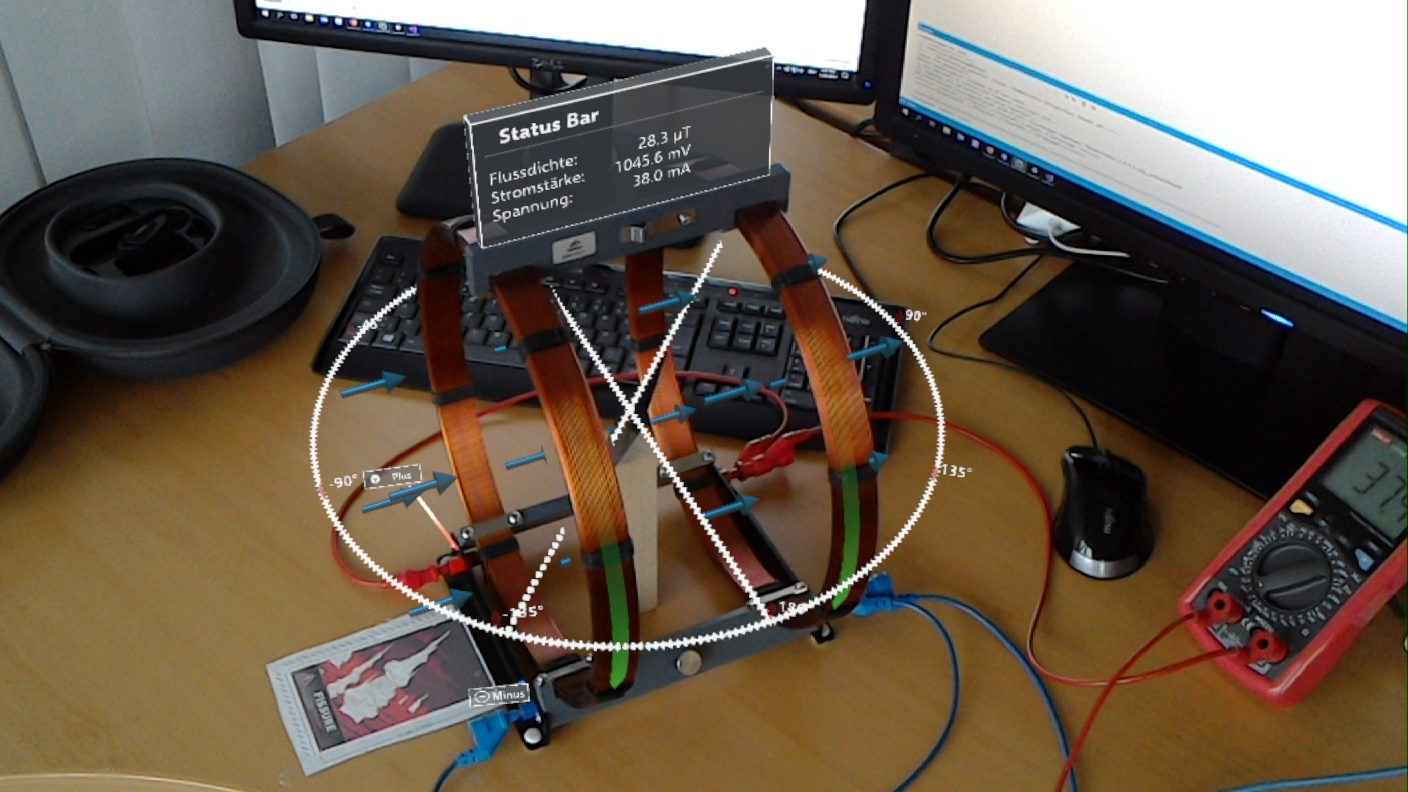
\includegraphics[width=\textwidth]{images/HL_SS1.jpg}

	\vspace{0.25cm}

	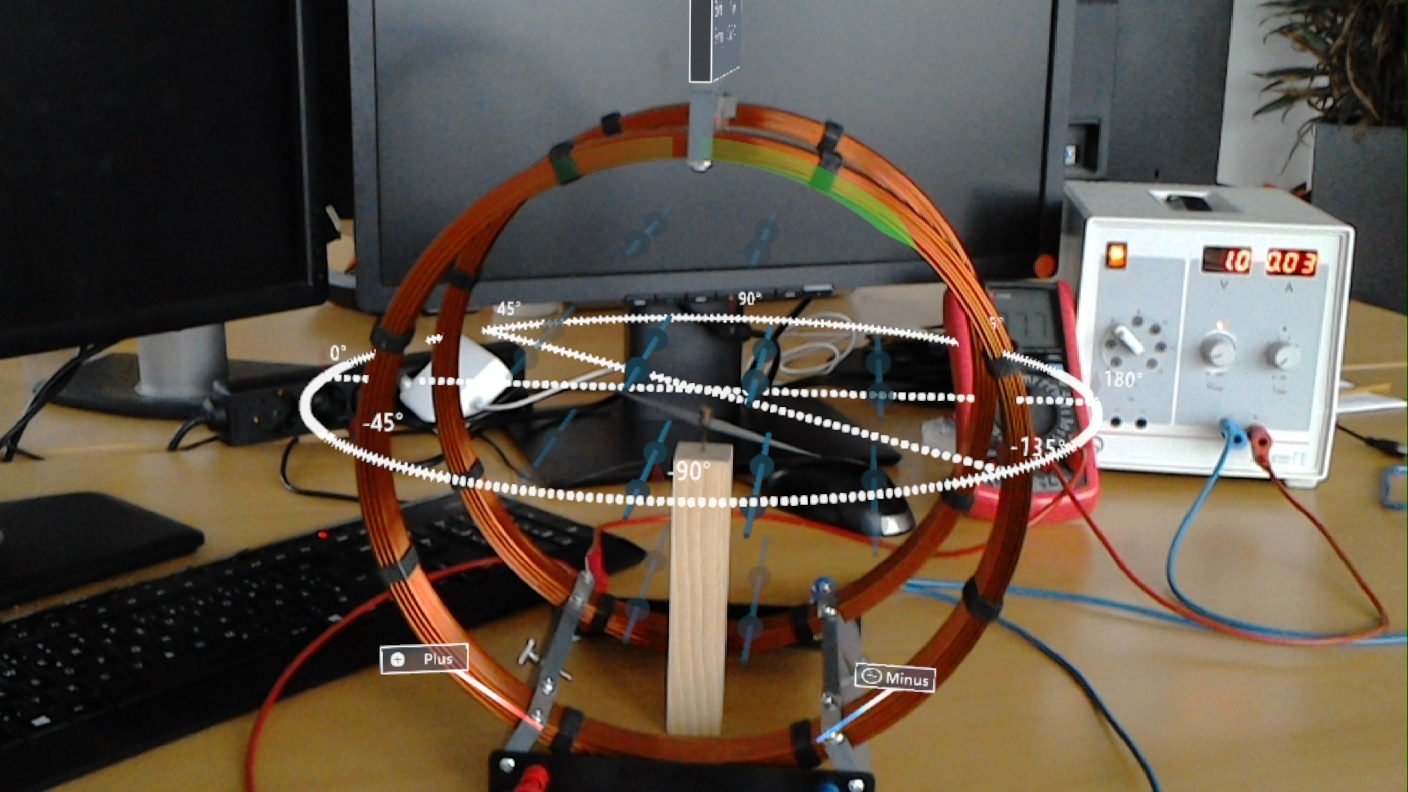
\includegraphics[width=\textwidth]{images/HL_SS2.jpg}
	\caption{Erster Eindruck HoloLens}
	\label{img:HL_SS_Intro}
\end{figure}

\subsubsection{Aufnahmen mit der HoloLens}
Zunächst ist festzuhalten, dass herkömmliche Screen-Captures auf der HoloLens nur eingeschränkt sinnvoll wären. Hier wären nämlich nur die gerenderten Objekte sichtbar, die so auch in einer Entwicklungsumgebung zu sehen sind. Die Nutzererfahrung entsteht jedoch durch das Zusammenspiel mit dem Hintergrund. Deshalb bietet die HoloLens eine angepasste Funktion, um möglichst das abzubilden, was der Nutzer tatsächlich sieht: Das \textit{Mixed Reality Capture (MRC)}.\\

Mit dem Mixed Reality Capture lassen sich Screenshots und Screen-Videos aufnehmen. Dazu nutzt die Brille ihre integrierte Frontkamera und überlagert deren Bild mit dem gerenderten Bild. So lässt sich besser darstellen, was ein Nutzer sieht. Allerdings bringt dieses Vorgehen mehrere Einschränkungen mit sich, durch die die Resultate von den tatsächlich wahrgenommenen Bildern abweichen. Damit die folgenden Bilder richtig eingeordnet werden können, sollen die wichtigsten Faktoren hier genannt werden.\\

Bei einem MRC-Foto ändert sich die Auflösung von 1268x720 (720p) zu 1408x792. Obwohl die Auflösung steigt ist damit dennoch ein wesentlicher Qualitätsverlust verbunden, da der Betrachter auf der HoloLens zwei HD-Bilder sieht (stereoskopisch), beim Foto aber nur ein Bild erzeugt wird. Außerdem geht die höhere Auflösung des Einzelbildes nicht mit einer höheren Pixeldichte einher, sondern mit einem größeren Sichtfeld. Ein Foto repräsentiert daher nicht die tatsächlichen Begrenzungen des FOV. Dazu kommt die Tranzparenz von Objekten. Diese hängt stark von der Farbe ab und entspricht nicht immer der Wahrnehmung des Nutzers. Farbige Objekte erscheinen auf Fotos stets etwas transparent, auch wenn sie den Hintergrund aus Sicht des Nutzers vollständig überdecken. Das trifft z.B. auf die blauen Objekte in den Fotos aus Abb. \ref{img:HL_SS_Intro} zu.\\

Darüber hinaus gibt es Faktoren, die durch ein Foto nicht abgedeckt werden können. Dazu gehören die schon erläuterten Eigenheiten der stereoskopischen Wahrnehmung. Auf einem Foto sieht ein Objekt immer scharf aus und es gibt keine Probleme mit der Akkommodation oder Konvergenz, auch wenn ein Nutzer diese möglicherweise erfährt. Außerdem nimmt ein Nutzer die Umgebung anders wahr als auf einem Foto, da das Sichtfeld (auf die Umgebung) kaum eingeschränkt wird und nicht in Farbe und Auflösung begrenzt ist, sondern direkt wahrgenommen wird.\\

Diese Faktoren gilt es beim Einsatz von solchen Screen-Captures zu berücksichtigen. Prinzipiell sind auch Aufnahmen möglich, die näher an die tatsächliche Nutzererfahrung heranreichen, diese erfordern aber weiteres Equipment, das im Rahmen dieser Arbeit nicht zur Verfügung steht.

\subsubsection{Allgemeines}
Spulenachse ist die Z-Achse.
\vspace{8px}
\begin{center}
	\fbox{
		\parbox{0.9\linewidth}{
			\vspace{4px}
			\textbf{Überblick}
			\begin{itemize}[rightmargin=12px, topsep=-12px]
				\setlength{\itemsep}{-1pt}
				\singlespacing
				\item Spule maßstabsgetreu modelliert mit ca. 2mm größerer Ausdehnung für Verdeckungsberechnung
				\item Rendering der Spule ausschließlich in den Z-Puffer
				\item Near Plane Fading verbirgt Objekte, die eine minimale Distanz zur Kamera unterschreiten
			\end{itemize}
			\vspace{18px}
	}}\\
\end{center}
\vspace{6px}

\textit{Occlusion Berechnung}\\
Nachmodelliert besser als Mesh, denn Mesh zu ungenau, Rendering nur in z puffer verbessert Performance, folgt Hinweis der Doku, near plane clipping beachten \\
\begin{figure}[H]
	\centering
	\includegraphics[width=0.45\textwidth]{images/todo.jpg}
	\hspace{0.05cm}	
	\includegraphics[width=0.45\textwidth]{images/todo.jpg}
	\caption{HoloLens Mesh vs. Modell}
	\label{img:mesh-vs-model}
\end{figure}

\begin{comment}
\begin{itemize}
	\item Für Verdeckung werden maßstabsgetreu nachmodellierte, virtuelle Objekte verwendet
	\item 3D Mesh in Blender erstellt, 2mm größer als echte Objekte für Spielraum
	\item Objekte werden möglichst genau über reale gelegt
	\item Rendering erfolgt ausschließlich in den Z-Puffer, dadurch sind die realen Objekte sichtbar, die virtuellen verdecken jedoch dahinterliegende, vrituelle Objekte
	\item Das Near Clipping Plane muss dafür jedoch sehr nah am Kameraursprung liegen, andernfalls würden weiter entfernte, virtuelle Objekte plötzlich doch vor realen Objekten angezeigt werden, sobald letztere zu nah sind und das Clipping die Objekte vom Rendering ausschließt
\end{itemize}
\end{comment}

\textit{Near Plane Fading}\\
Minimale Distanz, angenehmer als Clipping, fade to transparent nicht umgesetzt\\
\begin{comment}
\begin{itemize}
	\item Minnimum Distanz
	\item Behinderung bei Interaktion mit Versuchsaufbau
	\item Bessere UX als Clipping
	\item MRTK Standard Shader implementiert Fade To Black
	\item Shader auf Fade to transparent abgeändert
	\item Lineares Fading überall genutzt
\end{itemize}
\end{comment}

\textit{Künstliche Beleuchtung}\\
Beleuchtung bildet grob erwartete Lichtverhältnisse nach, keine Schatten\\
\begin{comment}
\begin{itemize}
	\item Virtuelle Beleuchtung von Oben bildet echte Lichtverhältnisse grob nach
	\item Unterstützt die Einbettung der 3D Objekte im Raum
\end{itemize}
\end{comment}

\subsubsection{Das Magnetfeld}
Die Darstellung des Magnetfeldes erfolgt über 3D-Geometrie, außer im Falle der Simulationsdaten. Die Geometrie wurde mit Blender erstellt und in Unity importiert. Die Fotos in Abb. \ref{img:mfield-result} zeigen die beiden alternativen Darstellungsmodelle.

\begin{figure}[H]
	\centering
	\includegraphics[width=0.45\textwidth]{images/todo.jpg}
	\hspace{0.05cm}	
	\includegraphics[width=0.45\textwidth]{images/todo.jpg}
	\caption{Links Feldlinien Rechts Vektoren}
	\label{img:mfield-result}
\end{figure}

\vspace{4px}
\begin{center}
	\fbox{
		\parbox{0.9\linewidth}{
			\vspace{4px}
			\textbf{Überblick}
			\begin{itemize}[rightmargin=12px, topsep=-12px]
				\setlength{\itemsep}{-1pt}
				\singlespacing
				\item Feldlinien und Vektoren als 3D-Objekte modelliert
				\item Feldlinien sind Zylinder mit integrierten Pfeilköpfen zur Richtungsangabe
				\item Vektoren als Pfeile modelliert
				\item Durchmesser Zylinder/Pfeilkopf ca. 1cm/2cm, Länge der Objekte zwischen 3 und 15 cm
				\item Rasterisierung ist parametrisiert, konkreten Parameter aus praktischer Erfahrung bestimmt
				\item Form wird durch Schattierung betont
				\item Simulationsdaten als farbige Linien, umgesetzt über Low-Level Draw Calls
				\item Grün-Rot-Farbverlauf als Farbskala genutzt
			\end{itemize}
			\vspace{18px}
	}}\\
\end{center}
\vspace{6px}

\textit{Feldlinien}
Die Feldlinien der Spule verlaufen orthogonal auf der X-Y in Richtung der Z-Achse. Damit die gewünschten Eigenschaften (Stärke, Homogenität und Richtung) des dreidimensionalen Feldes anhand des Feldlinienmodells erkennbar sind, bedarf es mindestens vier Linien. In einer 2x2 Anordnung um den Mittelpunkt der X-Y-Ebene ist so der Abstand in beiden Dimensionen sichtbar und die Linien sind symmetrisch zur Z-Achse. Anhand der Parallelität lässt sich die Homogenität erkennen und anhand des Abstandes (in der horizontalen oder vertikalen, beide sind gleich groß) die Stärke. Die Flussrichtung ist über eingebaute Pfeilspitzen abgebildet.\\

Bei einem festen, für die Darstellungen zur Verfügung stehenden Volumen und kleiner werdenden Abständen müssen zunehmend mehr Linien gezeichnet werden. Zu viele Objekte würden jedoch die Sichtbarkeit anderer Elemente wie Magnetnadel und Kompass beeinträchtigen. Außerdem transportieren zusätzliche Feldlinien keine zusätzlichen Informationen. Allerdings unterstützt die Beobachtung, dass mit zunehmender Flussdichte die Anzahl der Feldlinien steigt, das Verständnis des Feldlinienmodells. Daher wurde für die Umsetzung das Interval von minimalem und maximalem Abstand so gewählt, dass mindestens 4 und höchstens zwölf Linien dargestellt werden. Als 

\begin{itemize}
	\item Mindestens 4 (2x2) (notwendig um Homogenität zu erkennen)
	\item Maximal 16 (4x4)
	\item Zylindrischer Ausschnitt gewählt mit $r=2/3 * R = 10 cm$
	\item Abstandsformel: 
	\item Dargestellte Größe: Flussdichte
\end{itemize}
Vektoren
\begin{itemize}
	\item Mindestens 8 (2x2x2) (notwendig um Homogenität zu erkennen)
	\item Gewählte Rasterisierung: 2x2x4
\end{itemize}
Simulation
\begin{itemize}
	\item Feldlinien
	\item Anzahl, Ebene und Ausrichtung
	\item Farbskala
\end{itemize}

\subsubsection{Der Stromfluss}

\subsubsection{Der Kompass}
\textbf{Kompass-Linien und Strom-Pfeile}
\begin{itemize}
	\item Darstellungen über 2D-Linien mit Unity's LineRenderer
	\item Für gestrichelte Linien eine Textur mit einem weißen Kreis und transparentem Hintergrund, dabei wird die Skalierung mit Tiling auf die Länge der Linie angepasst
	\item Strom-Pfeile haben Bilboard-Verhalten, Maßgebend ist dabei die Vorwärtsrichtung ihres Transform.
	\item Fade-Away-Effekt verhindert zu steile Winkel, so sind immer die relevanten Pfeile sichtbar
\end{itemize}

\subsubsection{Weitere Darstellungen}
\textbf{Textboxen}
\begin{itemize}
	\item Verwendung der im MRTK vorhandenen Schriftsätze
	\item Dunkelgrauer Hintergrund verbessert Lesbarkeit, da Text vor transparentem Grund vor einigen Hintergründen schwer zu lesen ist
	\item Dank leicht transparenter Hintergrund ist die Textbox nicht so dominant im Bild und die dahinterliegenden Objekte sind für den Nutzer noch sichtbar
	\item Umsetzung als 3D Objekt, damit wird Stabilisierung genutzt
\end{itemize}


\subsection{Interaktion}
\textbf{Erkennung der Position über eigene Szene in Zusammenarbeit mit dem Nutzer}
\begin{itemize}
	\item Nutzer versteht die Funktionsweise der Anwendung
	\item Nutzer erhält Feedback über den Prozess der Positionsbestimmung von der Anwendung
	\item Nutzer kann sein Verhalten anpassen und so den Prozess unterstützen
	\item Bessere Kalibrierung möglich
	\item Tracking nur für kurze Zeit erforderlich, das spart viel Ressourcen
	\item Marker verdeckt kein Teil des Sichtfeldes, kann nach Positionierung auch entfernt werden
\end{itemize}

\subsection{Performance}
Vorgenommene Optimierungen:
\begin{itemize}
	\item Single Pass Instanced rendering
	\item 16 bit depth buffer (min available)
	\item Vuforia nur für den Vorgang der Positionsbestimmung aktiv
	\item Physics Enginge deaktiviert
	\item Frustum Culling
	\item Occlusion Mesh wird auschließlich in Z-Puffer gerendert
	\item Texture MipMaps
\end{itemize}
